\documentclass{standalone}
\usepackage{graphicx}	
\usepackage{amssymb, amsmath, amsthm}
\usepackage{color}

\usepackage{tikz}
\usetikzlibrary{intersections, backgrounds}

\definecolor{light}{RGB}{220, 188, 188}
\definecolor{mid}{RGB}{185, 124, 124}
\definecolor{dark}{RGB}{143, 39, 39}
\definecolor{highlight}{RGB}{180, 31, 180}
\definecolor{gray10}{gray}{0.1}
\definecolor{gray20}{gray}{0.2}
\definecolor{gray30}{gray}{0.3}
\definecolor{gray40}{gray}{0.4}
\definecolor{gray60}{gray}{0.6}
\definecolor{gray70}{gray}{0.7}
\definecolor{gray80}{gray}{0.8}
\definecolor{gray90}{gray}{0.9}
\definecolor{gray95}{gray}{0.95}
\newcommand{\dd}{ \mathrm{d} }

\newcommand{\mcpoint}[2]{  
  \fill[color=dark] (#1, #2) circle (7pt); 
  \fill[color=light] (#1, #2) circle (5pt);
}

\begin{document}

\begin{tikzpicture}[scale=0.35, thick]
  \node[] at (26,-2) {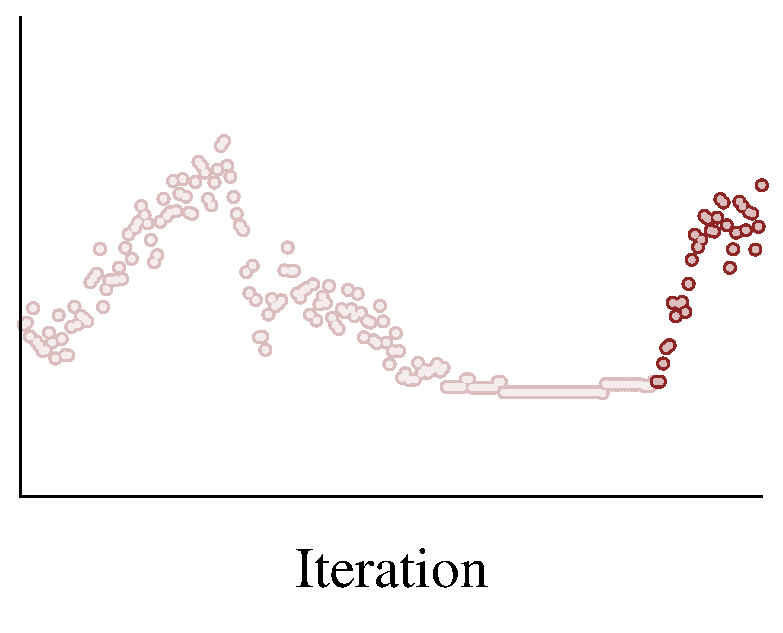
\includegraphics[width=8.4cm]{funnel_trace3.eps}};
  \node[rotate=90] at (14, -1) { $q_{2}$ }; 
\end{tikzpicture}

\end{document}  